\documentclass[a4paper]{article}

\addtolength{\hoffset}{-2.25cm}
\addtolength{\textwidth}{4.5cm}
\addtolength{\voffset}{-3.25cm}
\addtolength{\textheight}{5cm}
\setlength{\parskip}{0pt}
\setlength{\parindent}{0in}

%----------------------------------------------------------------------------------------
%	PACKAGES AND OTHER DOCUMENT CONFIGURATIONS
%----------------------------------------------------------------------------------------

\usepackage{blindtext} % Package to generate dummy text
\usepackage{charter} % Use the Charter font
\usepackage[utf8]{inputenc} % Use UTF-8 encoding
\usepackage{microtype} % Slightly tweak font spacing for aesthetics
\usepackage[english]{babel} % Language hyphenation and typographical rules
\usepackage{amsthm, amsmath, amssymb} % Mathematical typesetting
\usepackage{float} % Improved interface for floating objects
\usepackage[final, colorlinks = true,
            linkcolor = black,
            citecolor = black]{hyperref} % For hyperlinks in the PDF
\usepackage{graphicx, multicol} % Enhanced support for graphics
\usepackage{xcolor} % Driver-independent color extensions
\usepackage{marvosym, wasysym} % More symbols
\usepackage{rotating} % Rotation tools
\usepackage{censor} % Facilities for controlling restricted text
\usepackage{listings} % Environment for non-formatted code, !uses style file!
\usepackage{pseudocode} % Environment for specifying algorithms in a natural way
 % Environment for f-structures, !uses style file!
\usepackage{booktabs} % Enhances quality of tables
\usepackage{tikz-qtree} % Easy tree drawing tool
 % Configuration for b-trees and b+-trees, !uses style file!
\usepackage[backend=biber,style=numeric,
            sorting=nyt]{biblatex} % Complete reimplementation of bibliographic facilities
\addbibresource{ecl.bib}
\usepackage{csquotes} % Context sensitive quotation facilities
\usepackage[yyyymmdd]{datetime} % Uses YEAR-MONTH-DAY format for dates
\renewcommand{\dateseparator}{-} % Sets dateseparator to '-'
\usepackage{fancyhdr} % Headers and footers
\pagestyle{fancy} % All pages have headers and footers
\fancyhead{}\renewcommand{\headrulewidth}{0pt} % Blank out the default header
\fancyfoot[L]{} % Custom footer text
\fancyfoot[C]{} % Custom footer text
\fancyfoot[R]{\thepage} % Custom footer text
\newcommand{\note}[1]{\marginpar{\scriptsize \textcolor{red}{#1}}} % Enables comments in red on margin
\usepackage{mathtools}
\usepackage{amsmath}
\DeclarePairedDelimiter\abs{\lvert}{\rvert}%
\usepackage{cancel}
\usepackage{minted}
\usepackage{float}
\usepackage{caption}
\usepackage{subcaption}
%-------------------------------

%----------------------------------------------------------------------------------------

%-------------------------------
%	ENVIRONMENT SECTION
%-------------------------------
\pagestyle{fancy}
\usepackage{mdframed}

\usepackage[sfdefault]{FiraSans} %% option 'sfdefault' activates Fira Sans as the default text font
\usepackage[T1]{fontenc}
\renewcommand*\oldstylenums[1]{{\firaoldstyle #1}}


% remove numbering from sections
\usepackage{titlesec}
\titleformat{\section}{\normalfont\Large\bfseries}{}{0pt}{}



%-------------------------------------------------------------------------------------------
%	CUSTOM COMMANDS
%-------------------------------
\newcommand{\gaussian}{\frac{1}{\sigma\sqrt{2\pi}}\exp\left(- \frac{(x-\mu)^2}{2\sigma^2}\right)}
\newcommand{\R}{\mathbb R}

\def\inline{\lstinline[basicstyle=\ttfamily,keywordstyle={}]}


\begin{document}


%-------------------------------
%	TITLE SECTION
%-------------------------------

\fancyhead[C]{}
\hrule \medskip % Upper rule
\begin{minipage}{0.295\textwidth}
\raggedright
\footnotesize
Francisco Javier Sáez Maldonado \hfill\\
franciscojavier.saez@estudiante.uam.es
\hfill\\
\end{minipage}
\begin{minipage}{0.4\textwidth}
\centering
\large
Online Signature Lab Report\\
\normalsize
Deep Learning for Biometric Signal Processing\\
\end{minipage}
\begin{minipage}{0.295\textwidth}
\raggedleft
\today\hfill\\
\end{minipage}
\medskip\hrule

%-------------------------------
%	CONTENTS
%-------------------------------

\tableofcontents

\section{Introduction}

The objective of this session is to DEVELOP and EVALUATE an online signature recognition algorithm. According to the theory sessions, signature recognition systems can be divided into two categories:

\begin{itemize}
\item	Off-line: the input is a static image of the signature.
\item	On-line: the signature is acquired using a specific digital sensor which includes the static image and dynamic signals related with the way the signature was done: x,y coordinates and pressure as a function of time.
\end{itemize}

Figure \ref{fig:intro} shows a block diagram of a typical online signature recognition algorithm where [x,y,p] are the captured signals by the sensor (Cartesian coordinates and pressure), ft is the feature vector of the query signature to be compared with the fc feature vector of the signature stored in the database (claimed identity). 


In this session we will assume that the data is available (previously acquired) and we will focus on the development of two modules:
\begin{itemize}
\item	Feature Extraction Module.
\item	Matcher.
\end{itemize}
You must complete the tasks proposed in this document and answer the questions included. 

\begin{figure}[H]
  \centering
  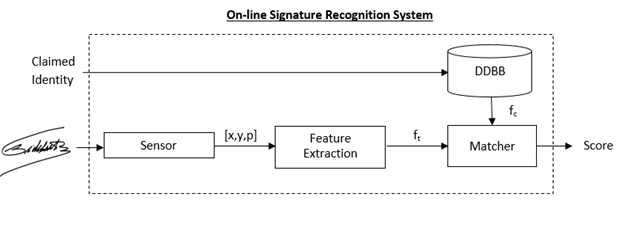
\includegraphics[scale=0.8]{Figures/Schema}
  
  \caption{Block Diagram of a typical online signature recognition system}
  \label{fig:intro}
\end{figure}

\section{Data}

For the practice we will use 50 users from the BiosecurID database. Each of the users have 28 signatures acquired in 4 sessions with a time lapse of 2 months. From the 28 signatures, 16 are genuine (4 per session) and 12 are forgers (3 per session). In this practice we will only consider the genuine signatures.

Each of the signatures is stored in .mat file which contains three vectors of same length with the x, y coordinates and the pressure as functions of time.
The formatting of the files is \inline{uXXXXsYYYY_sgZZZZ.mat}:

\begin{itemize}
\item XXXX: user number
\item	YYYY: session number
\item	ZZZZ: signature number
\end{itemize}

The GENUINE signatures of each session are those with \(ZZZZ=[0001,0002,0006,0007]\).The signatures with \(ZZZZ=[0003,0004,0005]\) are the FORGERS and they will NOT be used in this practice.


\subsection*{Drawing signals}
Choose a signature (from a random user) and show (assuming that the sensor has a \(200\) samples/second acquisition rate):
\begin{itemize}
\item	Signal x as a function of signal y.
\item	Signal x as a function of time.
\item	Signal y as a function of time.
\item	Signal p as a function of time.
\end{itemize}


 Firstly, we realise that we can read the data easily iterating through three \inline{for} loops and using a single line to read the file, by using \inline{sprintf(\'%02d\',user)}, which converts the user number to a 2 decimal number. This way, we can avoid the \inline{if} statement:

\begin{minted}{MatLab}
  for user=1:n_users
    for session = (1:4)
      for sign_genuine = (1:4)
          %This is how to load the signatures: 
          BiosecurID=load(['./DB/u100', sprintf('%02d',user) ,'s000', num2str(session), 
                                '_sg000', num2str(genuine_signs(sign_genuine)), '.mat']);
         
\end{minted}

Now, we created the script \inline{plot_signals.m} to load a selected user, session and sign and plot the four asked signals. In the first case, we selected \(user=7\), \(session=2\) and \(sign=1\). The result is shown in Figure \ref{fig:four:signals}:

\begin{figure}[H]
  \centering
  \subfloat{\label{fig:1a}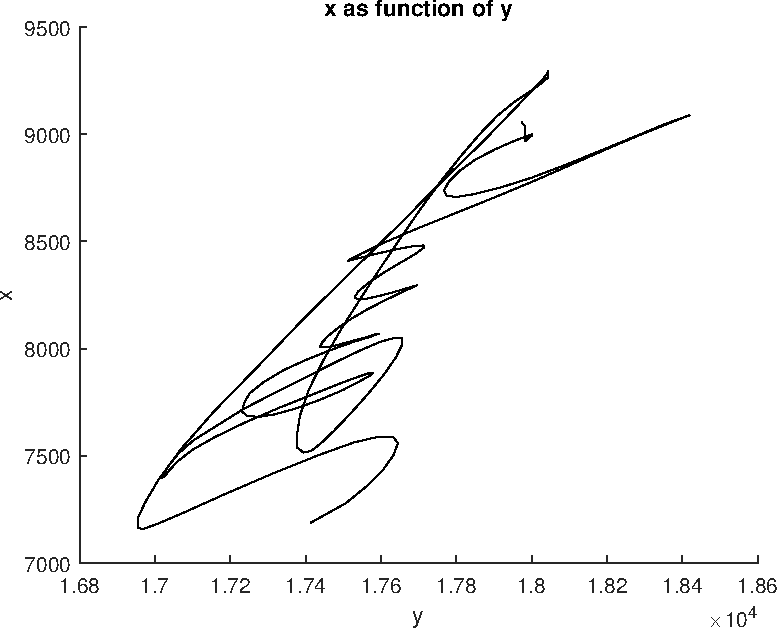
\includegraphics[width=0.35\linewidth]{Figures/x-func-y-1}}\qquad
  \subfloat{\label{fig:1b}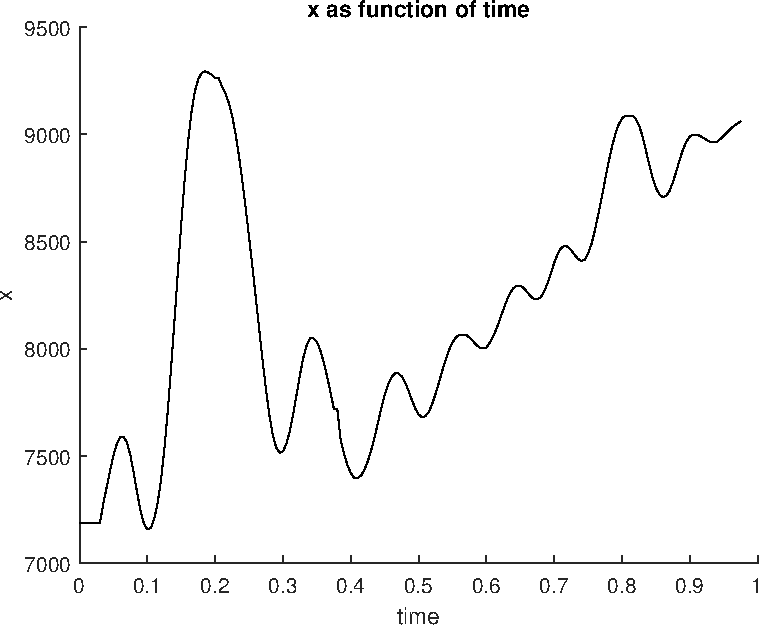
\includegraphics[width=0.35\linewidth]{Figures/x-func-t-1}}\\
  \subfloat{\label{fig:1c}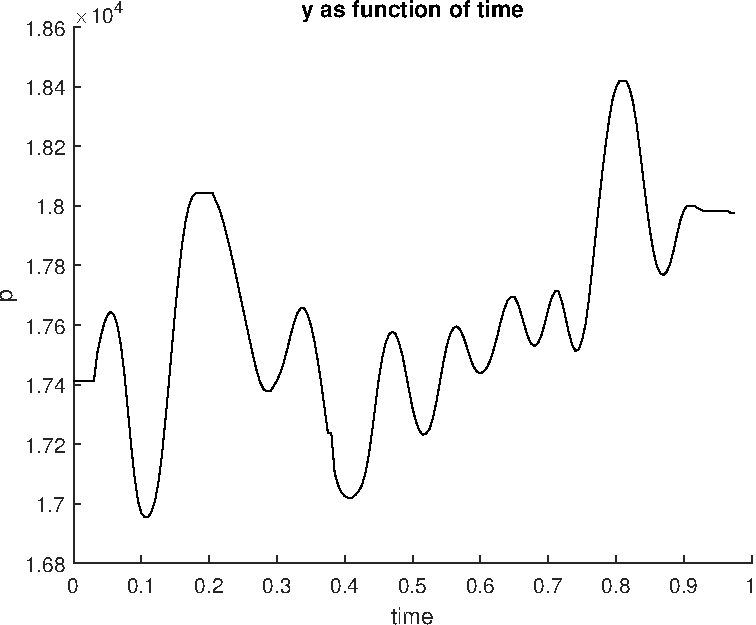
\includegraphics[width=0.35\textwidth]{Figures/y-func-t-1}}\qquad%
  \subfloat{\label{fig:1d}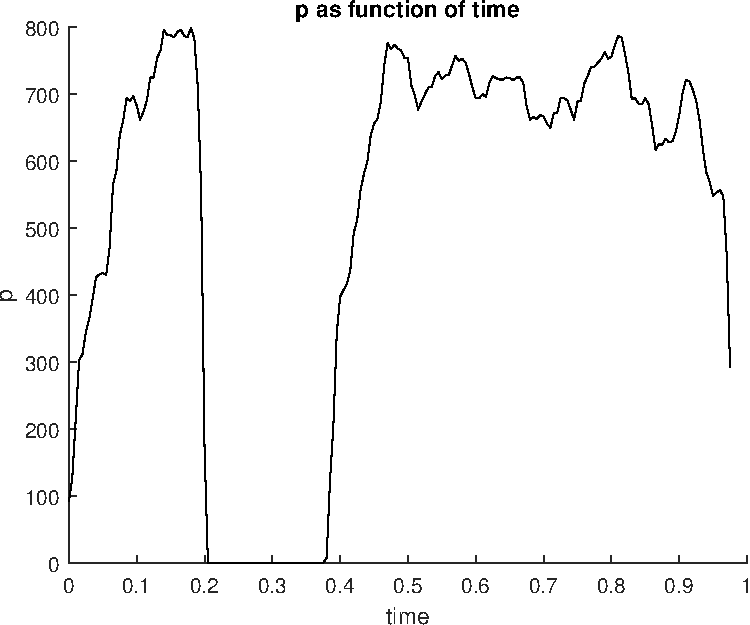
\includegraphics[width=0.35\textwidth]{Figures/p-func-t-1}}%
  \caption{Plot of $x$ as function of $y$, and then $x,y,p$ as functions of $t$.}
  \label{fig:four:signals}
\end{figure}

\subsection*{Repeat the process}

We repeat the process, using now \(session = 3\), \(sign=1\). We changed session to see if we can see any differences between different days.

\begin{figure}[H]
  \centering
  \subfloat{\label{fig:1a}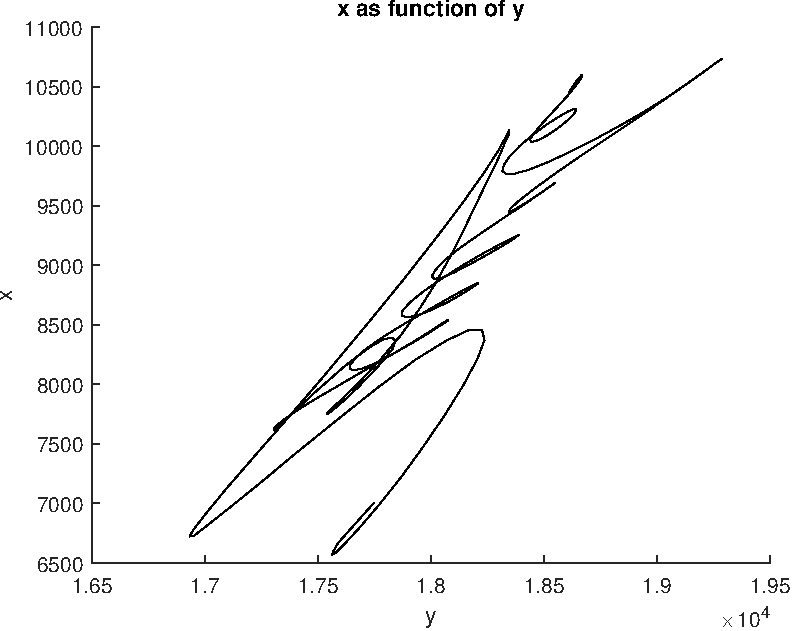
\includegraphics[width=0.35\linewidth]{Figures/x-func-y-2}}\qquad
  \subfloat{\label{fig:1b}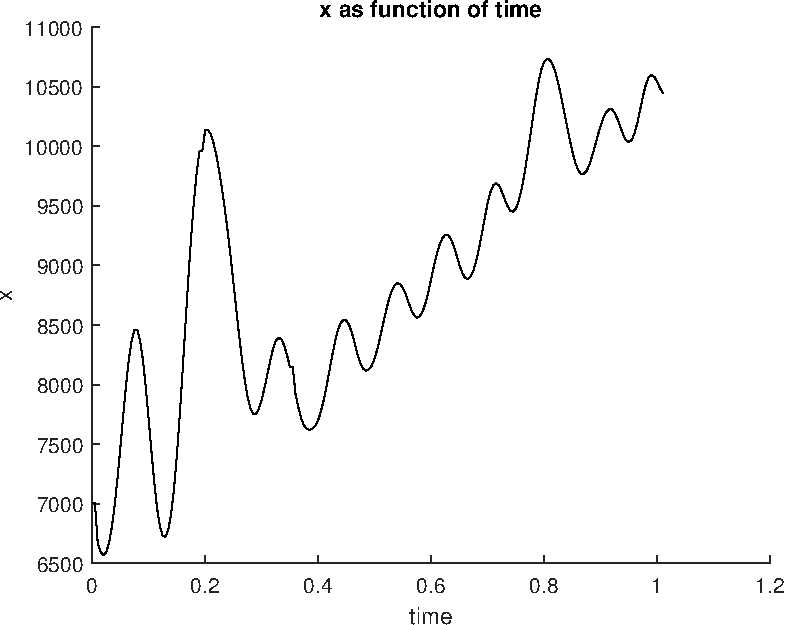
\includegraphics[width=0.35\linewidth]{Figures/x-func-t-2}}\\
  \subfloat{\label{fig:1c}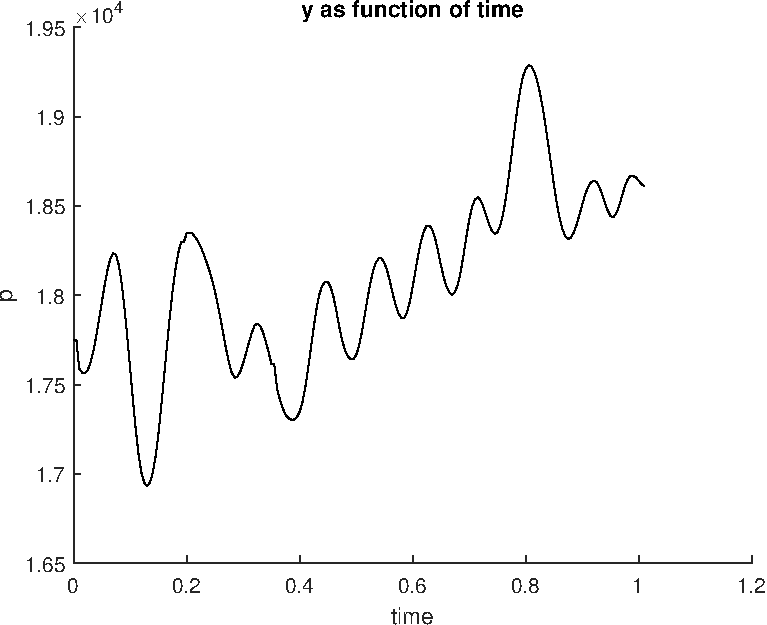
\includegraphics[width=0.35\textwidth]{Figures/y-func-t-2}}\qquad%
  \subfloat{\label{fig:1d}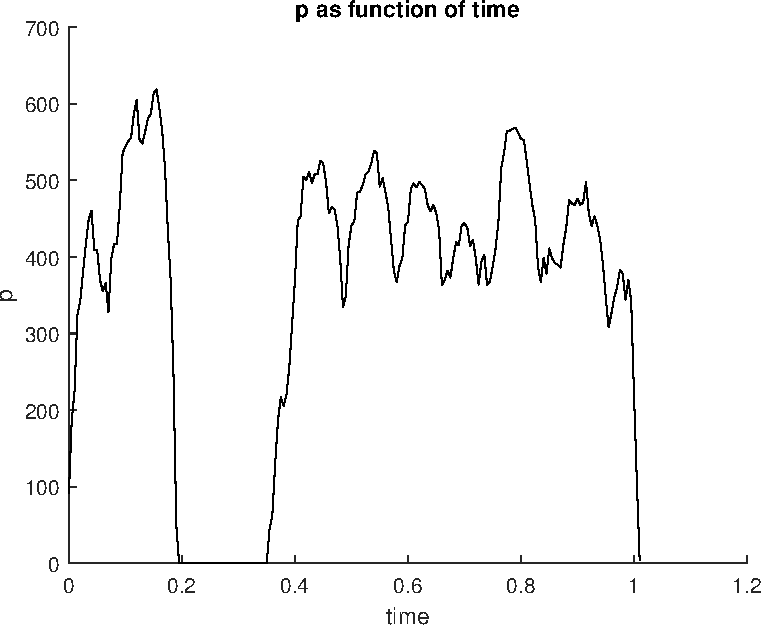
\includegraphics[width=0.35\textwidth]{Figures/p-func-t-2}}%
  \caption{Second sign. Plot of $x$ as function of $y$, and then $x,y,p$ as functions of $t$.}
  \label{fig:four:signals:2}
\end{figure}



\textbf{ Are the different signals reasonable? Do they have the same length? Why?}

We can see that the two signs are relatively similar. The second one is shifted to the left, but it has the same shape and similar lines. If we have a look at $x,y,p$ as functions of $t$, we can see that its shape, trend and \emph{ups and downs} are very similar in both signatures, which tells us that very similar processes have been followed to draw each of them. Hence, we can say that they are \textbf{reasonable}.\\

The signs do not have the same length neither in the $x,y$ axis nor in the $t$ axis. We see that the second sign was drawn quite bigger (approx $1.500$ difference) than the second one, and it also took approximately $0.2$ seconds longer to be drawn. The \textbf{explanation} of this is simple: the time for a person drawing its sign its variable and depends on many factors, and the difference between the times is maybe not noticeable for humans, but it is for the computers that works with exact numbers.

\section{Feature Extraction}


The comparison of signals with different lengths is not trivial. Therefore, we will extract 4 global parameters of each of the signatures. So, each signature will be represented by a feature vector with fixed size equal to 4. These parameters are:

\begin{enumerate}
\item	Total duration of the signature: T
\item	Number of pen-up (number of times the pen was lifted). It means the number of times (not the number of samples) that p is equal to 0.
\item	Duration of pen-down (signal p is different to 0) Td divided by the total duration \(T:Td/T\)
\item	Average pressure in pen-down (signal p is different to 0).
\end{enumerate}
You have to develop 4 functions to extract each of the parameters: 
\begin{enumerate}
  \item	\inline{T=Ttotal(x)}
  \item	\inline{Npu=Npenups(p)} 
  \item \inline{Tpd=Tpendown(p)}
  \item	\inline{Ppd=Ppendown(p)}
\end{enumerate}

According to those functions, we will develop a new function with input data \((x,y,p)\) of a given signature and output data the feature vector containing the 4 parameters (\inline{FeatVect=featureExtractor(x,y,p)}).
Based on your function featureExtractor you have to develop a program (\inline{ProcessBiosecurID.m}) to extract all the feature vectors from the database and store it in a matrix with 3 dimensions:

\begin{itemize}
\item	Dimension 1: number of user (1:50)
\item	Dimension 2: number of signature (1:16)
\item Dimension 3: number of parameter (1:4)
\end{itemize}

You have to save this matrix into the file \inline{BiosecurIDparameters.mat}.\\

Once you have the file \inline{BiosecurIDparameters.mat}, you have to plot the distributions normalized between 0 and 1 (dividing by the total number of points of the distribution) for each of the 4 parameters. \\
\emph{HINT: You can use the Matlab functions hist.m and histc.m}\\

\textbf{Comments about the developed code for the feature extraction.}

The four implemented functions were implemented in files with the same name as they are called in the file \inline{featureExtractor.m}. The functions are pretty simple: all of them but one are coded in \textbf{1 line}. The one that is a little bit longer is \inline{Npenups}. In this function, we have to take into account that if we find a zero in the \emph{pressure function}, we have to check if the previous position was \textbf{not} a zero. To achieve this, we find where the function is equal to zero and we loop over those index and check if the previous position was (or not) a zero.

To be able to code the rest of the functions in one line, \emph{logical indexing} was very useful. This allows us to index the elements of a vector that match a condition. For instance, in the case of \inline{Ppendown}, which computes the mean pressure when the pen is down, it is useful to use \inline{p(p>0)} which selects from \(p\) the positions where it is greater than zero. Using this, the complete function is:

\begin{minted}{MatLab}
function Ppd = Ppendown(p)
  % Compute mean pressure using positions 
  % Where pen is down (p > 0)
  Ppd = mean(p(p > 0) );
end
\end{minted}

\textbf{QUESTION:  Plot the 5 distributions.}


\section{Performance Evaluation}

We will evaluate the performance of our system according to the number of signatures N in the enrollment set \((N=1, N=4 \) and \(N=12)\).\\

The similarity score between a query/test signature and the enrollment signatures (signatures in the database) will be the Euclidean distance between feature vectors (vectors with 4 parameters).  The final score will be the average score of the N comparisons (comparison between the query/test sample and the N enrollment samples).\\

You have to develop the function \inline{Score=Matcher(test,Model)} where:
\begin{itemize}
\item	Score: is the final score of the comparison.
\item	test: is the feature vector of the query/test signature \((1\times4)\)
\item	Model: is a matrix containing the feature vectors of the signatures enrolled in the database. Therefore, this matrix contains Nx4 values in which N is the number of signatures enrolled for the claimed identity.
\end{itemize}
There are two cases to be analyzed:
Genuine Scores: scores obtained when you compare a signature with his real enrolled identity (claimed identity = enrolled identity). So these users should be accepted by the system. For each user you will use N signatures as enrolled samples and the rest for testing:
\begin{enumerate}
\item	For \(N=1\) we will have \(SG=15\) genuine scores.
\item	For \(N=4\) we will have \(SG=12\) genuine scores.
\item	For \(N=12\) we will have SG=4 genuine scores.
\end{enumerate}
For each of the scenarios \((N=1,4,12)\) you have to save all the genuine scores into a matrix (with dimension \(50 \times SG)\). Each of the three matrixes will be stored into a .mat file with name: \inline{GenuineScores_N.mat}.\\

Impostor Scores: scores obtained when you compare a signature with the enrolled samples of other users (claimed identity $\neq$ enrolled identity). So these users should be rejected by the system. In this case, we will compare one signature of each user (the first one) with the models of the rest of the users (excluding the genuine case). Therefore, we will obtain SI=49 impostor scores for each user and each scenario \((N=1,4,12)\).
For each scenario \((N=1,4,12)\) these impostor scores will be saved into a matrix with dimensions \(50\times SI\), \((50x49)\). Each of the three matrixes will be stored into a .mat file with name: \inline{ImpostorScores_N.mat}.

Once we obtain the genuine and impostor scores, we will evaluate the performance of our system for each of the three scenarios \((N=1,4,12)\) as a function of: FAR/FRR, EER and DET curves.
To obtain these performance metrics you will have available the next functions:



\inline{[EER]=Eval_Det(GenuineScores, ImpostorScores, 'b')}, where the parameters are
\begin{enumerate}
\item	EER: value of the Equal Error Rate (error when FAR and FRR are equal)
\item	\inline{GenuineScores}: the scores from target or genuine comparisons. These scores are obtained after applying the following normalization: \(GenuineScores = 1./(GenuineScores_N+0.00000001)\)
\item	\inline{ImpostorScores}: the scores form non target or impostor comparisons. These scores are obtained after applying the following normalization: \(ImpostorScores =1./(ImpostorScores_N+0.00000001)\)
\end{enumerate}

\textbf{QUESTION. Plot the performance graphics (DET curves) using the genuine and impostors score stored in their respectively matrixes (for each of the scenarios \(N=1,4,12\)). Indicate the EER value.}


\textbf{QUESTION. According to the results, are they reasonable? What metrics are more illustrative? When do you obtain the best performance? }


\section{Extra}

\subsection{Extra work 1}
 If you want to obtain a mark up to 8 points out of 10 you should complete one of the following points:
 \begin{enumerate}
\item Think and give a reasonable explanation of some additional features you can extract from the signatures. Program them, and repeat the point 4. Performance Evaluation in order to prove their improvement in the system performance. 
\item 	Obtain a list of the most discriminative features and based on that make combinations of features in order to obtain a better performance.
\item 	Make an evaluation using the skilled forgeries signatures and compared the results with the random forgeries.
 \end{enumerate}

 \subsection{Extra work 2}
Extra work 2: If you want to obtain a mark up to 10 points out of 10 you should do the following (directly, without doing the Extra work 1):

\begin{enumerate}
  \item 	Develop an online signature recognition system based on local features (time functions) and Dynamic Time Warping for the Matcher. Repeat the same experimental protocol followed in the practice but using this new signature recognition system.
  \item 	You should use the following local features (time functions): x, y, pressure, (and their corresponding first and second derivative).
  \item 	You can use the DTW matcher available in Matlab. Take into account that it only allows to compare time functions of different lengths 1 to 1, i.e., x1 vs x2, y1 vs y2, etc. Therefore, you should compare time functions 1 to 1 and finally obtain the average between all time functions in order to obtain the final score of the comparison between two signatures.
  \item 	The equation to obtain the score of the 1vs1 time function comparison is score=e-D/k, where D is the minimum accumulative distance obtain after using DTW in Matlab, and K is the number of aligned time samples.
\end{enumerate}

\end{document}